\documentclass[11pt]{article}
\usepackage[T1]{fontenc}

\usepackage{graphicx}
\graphicspath{ {./figs/} }
\usepackage{hyperref}
\usepackage{listings}
\hypersetup{colorlinks=true}
\usepackage[margin=1in]{geometry}
\usepackage{amsmath}
\usepackage[parfill]{parskip}
\usepackage{bigints}
\usepackage{titling}

\usepackage{xspace}                    %%% correct spacing self-defined macros
\xspaceaddexceptions{[]}
\newcommand{\M}{\mathcal{M}}
\newcommand{\eps}{\epsilon}
\newcommand{\tauo}{\tau_{1}}
\newcommand{\taut}{\tau_{2}}
\newcommand\ddfrac[2]{\frac{\displaystyle #1}{\displaystyle #2}}
\newcommand{\e}{\mathrm{e}}

\newcommand{\mO}{\mathcal{O}}
\author{Alexander P Long}

\newcommand{\ii}{\mathrm{i}}
\newcommand{\tr}{\mathrm{tr}}
\newcommand{\T}{\mathrm{T}}

\newcommand{\deint}[2]{\dd^{#1}\;\!\! #2\;}
\newcommand{\deintdim}[2]{\frac{\dd^{#1}\;\!\! #2}{(2\pi)^{#1}}\;}
\newcommand{\dedreix}{\dd^{3}\:\!\! x\;}
\newcommand{\dedreiy}{\dd^{3}\:\!\! y\;}

\renewcommand{\deg}{\circ}

\newcommand{\de}{\partial}

% The following construct adds a bit of space to the end of a vector, so that
% the vector arrows do not collide with subscript like ² and '
\newcommand{\vectorwithspace}[1]{\vec{#1}\mkern2mu\vphantom{#1}}
\newcommand{\vect}[1]{\vectorwithspace{#1}}

\newcommand{\grad}{\vectorwithspace{\nabla}}
\newcommand{\dev}{\vectorwithspace{\de}}
\newcommand{\bv}[1]{\vectorwithspace{#1}}

\newcommand{\av}{\vectorwithspace{a}}
\newcommand{\cv}{\vectorwithspace{c}}
\newcommand{\dv}{\vectorwithspace{d}}
\newcommand{\ev}{\vectorwithspace{e}}
\newcommand{\fv}{\vectorwithspace{f}}
\newcommand{\gv}{\vectorwithspace{g}}
\newcommand{\hv}{\vectorwithspace{h}}
\newcommand{\iv}{\vectorwithspace{i}}
\newcommand{\jv}{\vectorwithspace{j}}
\newcommand{\kv}{\vectorwithspace{k}}
\newcommand{\lv}{\vectorwithspace{l}}
\newcommand{\mv}{\vectorwithspace{m}}
\newcommand{\nv}{\vectorwithspace{n}}
\newcommand{\ov}{\vectorwithspace{o}}
\newcommand{\pv}{\vectorwithspace{p}}
\newcommand{\qv}{\vectorwithspace{q}}
\newcommand{\rv}{\vectorwithspace{r}}
\newcommand{\sv}{\vectorwithspace{s}}
\newcommand{\tv}{\vectorwithspace{t}}
\newcommand{\uv}{\vectorwithspace{u}}
\newcommand{\vv}{\vectorwithspace{v}}
\newcommand{\wv}{\vectorwithspace{w}}
\newcommand{\xv}{\vectorwithspace{x}}
\newcommand{\yv}{\vectorwithspace{y}}
\newcommand{\zv}{\vectorwithspace{z}}
\newcommand{\Av}{\vectorwithspace{A}}
\newcommand{\Bv}{\vectorwithspace{B}}
\newcommand{\Cv}{\vectorwithspace{C}}
\newcommand{\Dv}{\vectorwithspace{D}}
\newcommand{\Ev}{\vectorwithspace{E}}
\newcommand{\Fv}{\vectorwithspace{F}}
\newcommand{\Gv}{\vectorwithspace{G}}
\newcommand{\Hv}{\vectorwithspace{H}}
\newcommand{\Iv}{\vectorwithspace{I}}
\newcommand{\Jv}{\vectorwithspace{J}}
\newcommand{\Kv}{\vectorwithspace{K}}
\newcommand{\Lv}{\vectorwithspace{L}}
\newcommand{\Mv}{\vectorwithspace{M}}
\newcommand{\Nv}{\vectorwithspace{N}}
\newcommand{\Ov}{\vectorwithspace{O}}
\newcommand{\Pv}{\vectorwithspace{P}}
\newcommand{\Qv}{\vectorwithspace{Q}}
\newcommand{\Rv}{\vectorwithspace{R}}
\newcommand{\Sv}{\vectorwithspace{S}}
\newcommand{\Tv}{\vectorwithspace{T}}
\newcommand{\Uv}{\vectorwithspace{U}}
\newcommand{\Vv}{\vectorwithspace{V}}
\newcommand{\Wv}{\vectorwithspace{W}}
\newcommand{\Xv}{\vectorwithspace{X}}
\newcommand{\Yv}{\vectorwithspace{Y}}
\newcommand{\Zv}{\vectorwithspace{Z}}
\newcommand{\sigv}{\vectorwithspace{\sigma}}
\newcommand{\epsv}{\vectorwithspace{\epsilon}}

\newcommand{\kpv}{\kv'}
\newcommand{\qpv}{\qv'}

\newcommand{\mpi}{\ensuremath{m_\pi}}
\newcommand{\mN}{\ensuremath{M_N}}
\newcommand{\mpiphys}{\ensuremath{m_{\pi\text{phys}}}}
\newcommand{\fpi}{\ensuremath{f_\pi}}
\newcommand{\ga}{\ensuremath{g_A}}
\newcommand{\gA}{\ensuremath{g_A}}
\newcommand{\fm}{\ensuremath{\mathrm{fm}}}
\newcommand{\dd}{\mathrm{d}}
\newcommand{\MN}{\ensuremath{M_\mathrm{N}}} % nucleon mass
\newcommand{\Mp}{\ensuremath{M_\mathrm{p}}} % proton mass

\newcommand{\calA}{\mathcal{A}} \newcommand{\calB}{\mathcal{B}}
\newcommand{\calC}{\mathcal{C}} \newcommand{\calD}{\mathcal{D}}
\newcommand{\calE}{\mathcal{E}} \newcommand{\calF}{\mathcal{F}}
\newcommand{\calG}{\mathcal{G}} \newcommand{\calH}{\mathcal{H}}
\newcommand{\calI}{\mathcal{I}} \newcommand{\calJ}{\mathcal{J}}
\newcommand{\calK}{\mathcal{K}} \newcommand{\calL}{\mathcal{L}}
\newcommand{\calM}{\mathcal{M}} \newcommand{\calN}{\mathcal{N}}
\newcommand{\calO}{\mathcal{O}} \newcommand{\calP}{\mathcal{P}}
\newcommand{\calQ}{\mathcal{Q}} \newcommand{\calR}{\mathcal{R}}
\newcommand{\calS}{\mathcal{S}} \newcommand{\calT}{\mathcal{T}}
\newcommand{\calU}{\mathcal{U}} \newcommand{\calV}{\mathcal{V}}
\newcommand{\calW}{\mathcal{W}} \newcommand{\calX}{\mathcal{X}}
\newcommand{\calY}{\mathcal{Y}} \newcommand{\calZ}{\mathcal{Z}}
\newcommand{\MeV}{\,\mathrm{MeV}}
\newcommand{\ppv}{{\pv'}}
\newcommand{\pp}{{p'}}
\newcommand{\ppx}{{p'_x}}
\newcommand{\ppy}{{p'_y}}
\newcommand{\ppz}{{p'_z}}
\newcommand{\p}{\partial}
\newcommand\tab[1][0.75cm]{\hspace*{#1}}
\title{Neutral Pion Photoproduction}
\begin{document}

\maketitle
\subsection{Lenkewitz convention vs ours}
Lenkewtiz calls the incoming momenta of the particles $\vec{k_1}$ and
$\vec{k_2}$, so to transfer that convention to our convention we use:
\begin{align}
	 & \vec{k}_1 =\vec{p} - \vec{k}/2       \\
	 & \vec{k}_2 =-\vec{p} - \vec{k}/2      \\
	 & \vec{k}'_1= \vec{p}\,' - \vec{k}'/2  \\
	 & \vec{k}'_2= -\vec{p}\,' - \vec{k}'/2
\end{align}
Throughout this document I will stick to the conventions present in
the BKM review, link here:
\href{https://arxiv.org/pdf/hep-ph/9501384}{https://arxiv.org/pdf/hep-ph/9501384}.
In particular I'm pretty sure the BKM review uses $F=2 f_\pi$
Here are a list of the Feynman rules used, as they are listed in the
BKM review, along with their equation number, using:\par
\makebox[1.5cm]{$l$} Momentum of a pion or nucleon propagator\\
\makebox[1.5cm]{$k$} Momentum of an external vector or axial source\\
\makebox[1.5cm]{$q$} Momentum of an external pion\\
\makebox[1.5cm]{$\epsilon$} Photon polarization vector\\
\makebox[1.5cm]{$\epsilon_A$} Polarization vector of an axial source\\
\makebox[1.5cm]{$p$} Momentum of a nucleon in a heavy mass formulation\\
\makebox[1.5cm]{$v_\mu$} nucleon 4-velocity\\
\makebox[1.5cm]{$S_\mu$} covariant spin-vector of the nucleon\\
And the pion isospin indices are $a,b,c$, and \par
Pion propagator (A.1)
\begin{equation}
	\ddfrac{i \delta^{ab}}{l^2-\mpi^2+i0}
\end{equation}
1 pion ($q$ out) A.12
\begin{equation}
	\frac{g_A}{F} S \cdot q \tau^a
\end{equation}
2 pions ($q_1$ in $q_2$ out) A.14
\begin{equation}
	\frac{1}{4 F^2} v \cdot (q_1 + q_2) \epsilon^{abc} \tau^c
\end{equation}
1 pion 1 photon where $a$ is the isospin of the outgoing pion A.15
\begin{equation}
	\frac{i e \ga}{F} \epsilon \cdot S \epsilon^{a3b} \tau^b
\end{equation}
1 pion ($q$ out) A.12
\begin{equation}
	\frac{\ga}{F} S \cdot q \tau^a
\end{equation}
2 pions, photon A.6
\begin{equation}
	e \epsilon^{a3b} \epsilon \cdot \left( q_1 +q_2 \right)
\end{equation}
Note $\epsilon=(0,\vec{ \epsilon}\;)$, where the zeroth element has
been set to zero with a choice of gauge.
Neglecting relativistic effects $S=(0, \vec{\sigma}/2)$.
So then
$\epsilon \cdot S =-\frac{\vec{\sigma}}{2} $
\section{Two Body Scattering}
The kinematic pre-factor is:
\begin{equation}
	K_{1N}= \frac{M_N +\mpi}{m_{3N}+\mpi} \frac{m_{3N}}{m_N}
\end{equation}
\subsection{Diagram A}
\begin{center}
	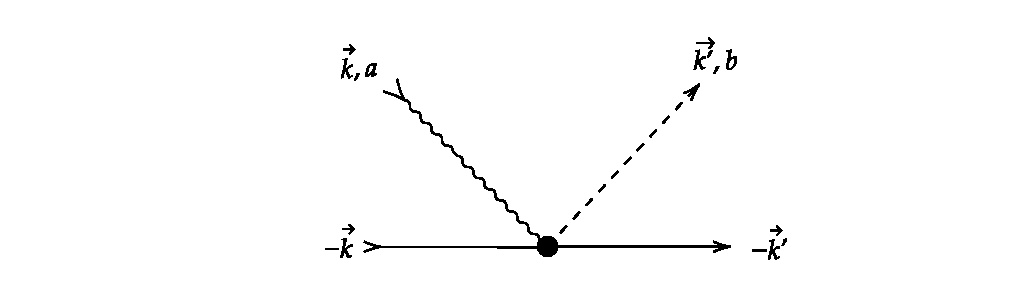
\includegraphics[scale=0.7]{1B-diagA.pdf}
\end{center}
This is just BKM A.15, with $a=15$
\begin{align}
	\calM & = \frac{i e \ga}{F} \epsilon \cdot S \varepsilon^{a3c}\tau^c    \\
	      & =-\frac{i e\ga}{2F} \epsilon \cdot \sigv\varepsilon^{33c}\tau^c
\end{align}
Note that $\varepsilon^{33c}\tau^c=0$ since $ \varepsilon^{33c}=0\, \forall\, c$, but this doesn't make sense to me, since it should mean this diagram is zero.
A.28 is the other diagrams that is 1 pion and photon, note that I am not sure what mass it is referring to by $m$
\begin{align}
	\calM & =-\frac{e \ga}{2m F} S \cdot \epsilon v \cdot k' (\tau^3 +1)                                    \\
	      & =\frac{e \ga}{4m F} \epsv \cdot \sigv \left(\sqrt{\mpi^2 +\kv'^2}-\vv\cdot\kv\right) (\tau_3+1) \\
	      & \approx\frac{e \ga}{4 F} \epsv \cdot \sigv \sqrt{\mpi^2 +\kv'^2}\, (\tau_3+1)
\end{align}
Now lets assume $m=\mpi$ and take the threshold limit $\kv'\to\vec{0}$, then we have
\begin{align}
	\calM & =\frac{e \ga}{4 F} \epsv \cdot \sigv \left( \tau_3 + 1 \right)
\end{align}
Which is the same as Lenkewitz diagrams a and b added together modulo some pre-factors.

\section{Three Body Scattering}
Lenkewitz uses the pre-factor
\begin{equation}
	K_{2N}= \frac{1}{(2\pi)^3} \ddfrac{m_\pi m_{3N}}{m_\pi+m_{3N}}
	\ddfrac{ e \ga}{4  f_\pi^3} \frac{1}{(4\pi)}
\end{equation}
Where $m_{3N}$ refers to the mass of the target $m_t$, so with that motivation, let
\begin{equation}
	\mu = \frac{1}{(2\pi)^3}
	\ddfrac{
		\mpi  m_t
	}{
		\mpi +m_t
	}
\end{equation}
\subsection{Diagram A}
\begin{center}
	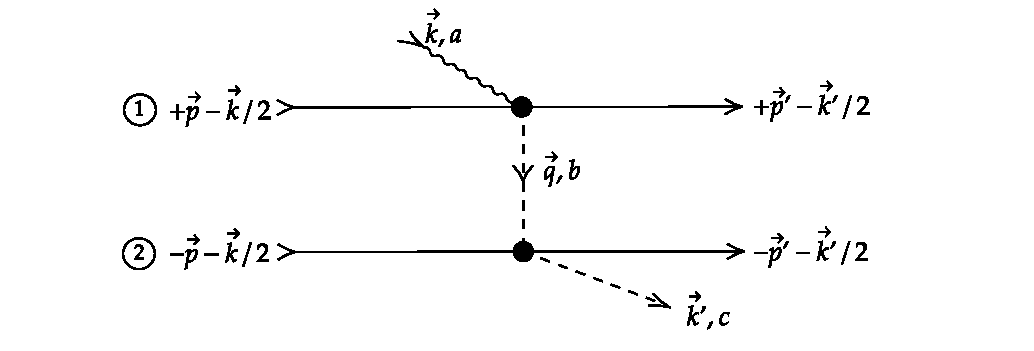
\includegraphics[scale=0.9]{2B-diagA.pdf}
\end{center}
From top to bottom we have
\begin{align}
	\calM_{1\to2} & =\mu \left[ i e \frac{\ga}{F} {\epsilon} \cdot {S}_1
		\epsilon^{b3d} \tau_1^d  \right]
	\left[ \ddfrac{i}{q^2 -\mpi^2+i0 }  \right]
	\left[ \frac{1}{4 F^2} v \cdot \left( q + k' \right) \epsilon^{bce}
		\tau_2^e \right]
\end{align}
The momenta into $\vec{q}$ is
\begin{equation}
	\vec{q}=\left(\pv-\kv/2 \right) +\kv -\left(
	\pv'-\kv'/2\right)=\pv-\pv' +\frac{1}{2} (\kv-\kpv)
\end{equation}
The energy associated with the propagator is $q_0=E_1+k_0-E_1'$ and we have:~\\
\begin{align}
	E_1= \ddfrac{ \left( \pv - \kv/2 \right)^2}{2\MN} +\MN\qquad
	E_1'= \ddfrac{ \left( \pv' - \kv'/2 \right)^2}{2\MN} +\MN\qquad
	k_0= \omega
\end{align}
So then
\begin{align}
	q_0 & =E_1-E_1'+\omega                                     \\
	    & =\frac{1}{2\MN}\left[ \left( \pv - \kv/2 \right)^2 -
		\left( \pv' - \kv'/2 \right)^2\right]+\omega \label{qzero}
\end{align}
Now we let
\begin{align}
	 & q^2 =q_0^2 - \qv^2                                             \\
	 & v \cdot \left( q+k' \right)= q_0+k'_0 =q_0+\sqrt{\mpi +\kv'^2}
\end{align}
We may need to include the relativistic contributions of $v$ at higher order.

Now to evaluate the isospin dependence recall $\pi_0\implies c=3$,
and that the implicit sum is over $b, d,e=1,2,3$. This can be
evaluated with the following Mathematica code:
\begin{align}
	 & \epsilon=\text{LeviCivitaTensor[3]}\;                     \\
	 & c=3;                                                      \\
	 & \sum_{b=1}^3 \sum_{e=1}^3 \sum_{d=1}^3 \epsilon[[b,3,d]],
	\epsilon[[b,c,e]] \tau_{1,d} \tau_{2,e}                      \\
	 & =\tau _{1,1} \tau _{2,1}+\tau _{1,2} \tau _{2,2}          \\
	 & =\vec{\tau}_1 \cdot \vec{\tau}_2-\tau_{1,3} \tau_{2,3}
\end{align}
So placing the spin indices up, and the nucleon labeling down we have
\begin{align}
	\epsilon^{b3d} \epsilon^{bce} \tau_1^d \tau_2^e & =\vec{\tau}_1 \cdot
	\vec{\tau}_2-\tau_{1}^{3} \tau_{2}^{3}
\end{align}
We will leave everything in terms of $q_0$ since that expression is so long.
\begin{align}
	\calM_{1\to2} & =\mu \left[-i e \frac{\ga}{F} \frac{1}{2} {\epsilon}
		\cdot \sigma_1 \right]
	\left[ \ddfrac{i}{q^2 -\mpi^2+i0 }  \right]
	\left[ \frac{1}{4 F^2} v \cdot \left( q + k' \right) \right]
	\left(\vec{\tau}_1 \cdot \vec{\tau}_2-\tau_{1}^{3} \tau_{2}^{3}\right) \\
	              & =\mu\frac{e\ga}{8F^3}
	\ddfrac{q_0+\sqrt{\mpi^2 +\kv'^2}}{q_0^2-\qv^2 -\mpi^2+i0 }
	\left(\vec{\tau}_1 \cdot \vec{\tau}_2-\tau_{1}^{3} \tau_{2}^{3}\right)
	\vec{\epsilon} \cdot \vec{\sigma}_1
\end{align}

With $q_0$ given by eq.\ref{qzero} so the full result for scattering
off an $A$ body nucleus is:
\begin{equation}
	\calM=\binom{A}{2}\left(\calM_{1\to2}+\calM_{2\to1}\right)\\
\end{equation}
This gives the final result
\begin{equation}
	\calM= \mu\frac{e\ga}{8F^3} \binom{A}{2}
	\ddfrac{q_0+\sqrt{\mpi^2 +\kv'^2}}{q_0^2-\qv^2 -\mpi^2+i0 }
	\left(\vec{\tau}_1 \cdot \vec{\tau}_2-\tau_{1}^{3} \tau_{2}^{3}\right)
	\vec{\epsilon} \cdot \left(\vec{\sigma}_1 +\vec{\sigma}_2\right)
\end{equation}
And to program this we use:
\begin{align}
	\qv & =\pv-\pv'+\frac{1}{2}(\kv-\kv')                      \\
	q_0 & =\frac{1}{2\MN}\left[ \left( \pv - \kv/2 \right)^2 -
		\left( \pv' - \kv'/2 \right)^2\right]+\omega
\end{align}
\subsection{Reduction to the threshold case}
In the threshold case we have
\begin{align}
	\kv' & =(\mpi,\vec{0})                                                 \\
	q_0  & = \omega +\calO\left(\frac{1}{M_N}\right) = \mpi + \calO \left(
	\frac{1}{M_N}  \right)
\end{align}
Making these substitutions gives:
\begin{align}
	\calM & = -\mu\frac{e\mpi\ga}{4F^3}
	\ddfrac{\epsilon\cdot \left( \sigv_1 +\sigv_2 \right) }{\left(\pv-\ppv+ \kv/2\right)^2}
	\left(\vec{\tau}_1 \cdot \vec{\tau}_2-\tau_{1}^{3} \tau_{2}^{3}\right)
\end{align}
%%%%%%%%%%%%%%%%%%%%%%%%%%%%%%%%%%%%%%%%%%%%%%%%%%%%%%%%%%%%%%%%%%%%%%%%%%%%%%%%%%%%%%%%%%%%%%
%%%%%%%%%%%%%%%%%%%%%%%%%%%%%%%%%%%%%%%%%%%%%%%%%%%%%%%%%%%%%%%%%%%%%%%%%%%%%%%%%%%%%%%%%%%%%%
\subsection{Diagram B}
\begin{center}
	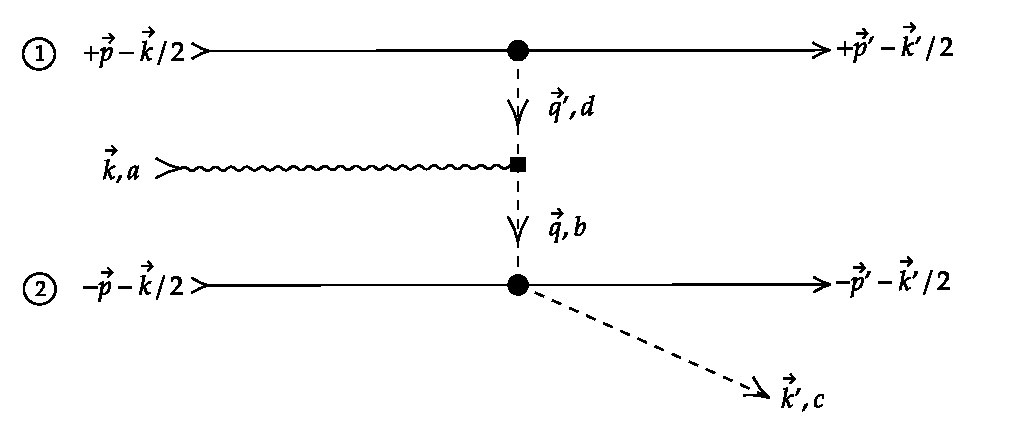
\includegraphics[scale=0.8]{2B-diagB.pdf}
\end{center}
If I recall correctly there is some weirdness on $q'$, such that $q'_0=0$.
This is probably because:
\begin{equation}
	q_0'=\frac{1}{2\MN}\left[ \left( \pv - \kv/2 \right)- \left( \pv' -\kv'/2 \right)^2\right] =\calO \left( 1/M_N \right)
\end{equation}
Again we will go from top to bottom, starting with A.12, then the
propagator, then A.6 etc. I will use $\epsilon$ for photon
polarization and $\varepsilon$ for the Levi-Civita tensor to avoid ambiguity.
\begin{align}
	\calM_{1\to2} & = \mu
	\left[ \frac{\ga}{F} S \cdot q' \tau_1^d\right]
	\left[ \ddfrac{i}{q'^2 -\mpi^2 +i0} \right]
	\left[ e \varepsilon^{d3b} \epsilon \cdot \left( q'+ q \right) \right]
	\left[ \ddfrac{i}{q^2 -\mpi^2+i0}  \right]\nonumber                        \\
	              & \times\left[ \frac{1}{4 F^2} v \cdot \left( q + k' \right)
		\varepsilon^{bce} \tau_2^e \right]
\end{align}
Note $c=3$ and:
\begin{align}
	\varepsilon^{b3e} \varepsilon^{d3b} \tau_1^d\tau_2^e & =
	-\tau_1^1\tau_2^1 - \tau_1^2 \tau_2^2                                                                          \\
	                                                     & = -(\vec{\tau}_1 \cdot \vec{\tau_2} -\tau_1^3 \tau_2^3)
\end{align}
See the Mathematica doc if you want a more general implementation.
Letting $\epsilon=(0,\epsv\,)$ and $v=(1,\vec{0})$ gives.
\begin{align}
	\calM_{1\to2} & = \mu
	\left[ \frac{-\ga}{2F} \qv'\cdot \sigv_1 \right]
	\left[ \ddfrac{-i e \epsv \cdot  \left(\qv' +\qv \right) }{q'^2-\mpi^2}  \right]
	\left[ \ddfrac{i}{q^2 -\mpi^2}  \right]
	\left[ \frac{1}{4 F^2}\left( q_0 + \sqrt{\mpi^2 +\kv'^2}\right) \right]                                \\
	              & \qquad\qquad\times \left[-1(\vec{\tau}_1 \cdot \vec{\tau_2} -\tau_1^3 \tau_2^3)\right] \\
	              & =\mu \ddfrac{e \ga }{8F^3}
	\ddfrac{
		\epsv \cdot \left( \qv+\qv' \right)\;
		\qv' \cdot  \sigv_1
	}{
		(q'^2-\mpi^2)
		(q^2 -\mpi^2)
	}
	\left( q_0 + \sqrt{\mpi^2 +\kv'^2}\right)
	(\vec{\tau}_1 \cdot \vec{\tau_2} -\tau_1^3 \tau_2^3)
\end{align}
So in an $A$ body nucleus the total contribution to the matrix element is
\begin{align}
	\calM & =\binom{A}{2}\left( \calM_{1\to2} +\calM_{2\to1}\right) \\
	      & =\mu\frac{e\ga}{8 F^3}
	\binom{A}{2}
	\ddfrac{
		\epsv \cdot \left( \qv+\qv' \right)\;
		\qv' \cdot\left(  \sigv_1 +\sigv_2\right)
	}{
		(q'^2-\mpi^2)
		(q^2 -\mpi^2)
	}
	\left( q_0 + \sqrt{\mpi^2 +\kv'^2}\right)
	(\vec{\tau}_1 \cdot \vec{\tau_2} -\tau_1^3 \tau_2^3)
\end{align}
Recall:
\begin{align}
	\qv' & =\pv-\pv' + \frac{1}{2} \left( \kv'-\kv \right)                                               \\
	q_0' & =\frac{1}{2\MN}\left[ \left( \pv - \kv/2 \right)- \left( \pv' -\kv'/2 \right)^2\right]        \\
	\qv  & =\qv'+\kv=\pv-\pv' + \frac{1}{2} \left( \kv'+\kv \right)                                      \\
	q_0  & =\frac{1}{2\MN}\left[ \left( \pv - \kv/2 \right)- \left( \pv' -\kv'/2 \right)^2\right]+\omega
\end{align}
\subsection{Reduction to the threshold case}
In the threshold case we have:
\begin{align}
	k'       & =(\mpi,\vec{0}),    \\
	q_0      & =\mpi'\approx\omega \\
	\qv+\qv' & =  2(\pv-\pv')
\end{align}
And for the time being we let $q_0'=0$ with the motivation being comparison to Lenkewitz. This gives:
\begin{align}
	\calM & = \mu \frac{e \mpi \ga}{4 F^3} \binom{A}{2}
	\ddfrac{ \qv' \cdot(\sigv_1 +\sigv_2) \epsv \cdot \left( \qv+\qv' \right)
	}{
		\qv^2 \left( \qv'^2+\mpi^2 \right)
	}
	(\vec{\tau}_1 \cdot \vec{\tau_2} -\tau_1^3 \tau_2^3) \\
	      & =\mu \frac{e \mpi \ga}{2 F^3} \binom{A}{2}
	\ddfrac{
		\left(\pv-\pv'-\kv/2 \right) \cdot \left( \sigv_2 +\sigv_2 \right) \epsv \cdot \left( \pv -\pv' \right)
	}
	{
		\left( \pv -\pv' + \kv/2 \right)^2
		\left[\left(\pv -\pv' - \kv/2\right)^2 + \mpi^2\right]
	}
	(\vec{\tau}_1 \cdot \vec{\tau_2} -\tau_1^3 \tau_2^3)
\end{align}
\section{Comparison to Lenkewtiz}
The literature for some reason always writes the result as diagram $A$ minus diagram $B$ which accounts for the difference in the negative sign.

We have already shown my results for 2 body diagrams A and B are the
same as Lenkewtiz up to a pre-factor. Lenkewtiz assigns
\begin{equation}
	K_{2N}= \frac{1}{(2\pi)^3} \ddfrac{m_\pi m_{3N}}{m_\pi+m_{3N}}
	\ddfrac{ e \ga}{4  f_\pi^3} \frac{1}{(4\pi)}
\end{equation}
Where Lenkewitz assigns $f_\pi= 93 \MeV$, and $g_A=1.26$. The BKM
review uses the same values.\par

The factor $3$ in the Lenkewitz paper comes from $\binom{A}{2}$.\\
The factor $1/(2\pi)^3$ comes from the integration measure.\\
The factor $m_\pi m_{3N}/(m_\pi+m_{3N})$ comes from kinematic considerations.\\
The factor $1/4\pi$ is a mystery, and is the  only term that I don't understand.~\\


I am off by a factor of 2 in both terms, perhaps this comes from an additional symmetry factor. Also, the sign on
diagram A doesn't match with Lenkewitz, but it is implemented with the negative sign, and reproduces the Lenkewitz
results.
~\\~\\

\section{Variable Substitution}
In the threshold case a variable substitution is used to remove the singularity. The kernel is proportional to:
\begin{align}
	\int \dd^3 p^\prime \frac{1}{
		\left( \pv -\pv^\prime - \frac{1}{2} \kv  \right)^2
	} f(\pv, \ppv)
	 & = \int \dd^3 q \frac{1}{\qv^2} f(\pv,\pv -\vec{\ell}- \kv/2) \\
	 & = \int \dd \Omega\; \dd \ell\;  f(\pv,\pv -\vec{\ell}- \kv/2)
\end{align}
With $\vec{q}=\pv-\ppv-\kv/2 \;\implies\; \ppv=\pv -\vec{q}- \kv/2 $.
This allows for the cancelation of the singularity in the threshold case.\\~\\

\subsection{Finite Energy}
At finite energy the situation is more complicated, we now have an integral of the form
\begin{equation}
	\int \frac{f(p,\pp)}{q_0^2- \left( \pv-\ppv-\kv/2 \right)^2 -\mpi^2	}
\end{equation}
We seek an additional transformation that eliminates the zero in the denominator.
\begin{align}
	\int \frac{f(p,\pp)}{q_0^2- \left( \pv-\ppv-\kv/2 \right)^2 -\mpi^2	} & =
	\int \dd^3 \pp \frac{f(p,\pp)}{q_0^2- \qv^2-m_\pi^2}\\
	 & =- \int \dd^3 \pp \frac{f(p,\pp)}{\qv^2 -\ell^2}\\
	 &= - \int \dd^3 u \frac{f(p,\pp)}{u^2} \\
	&= -\int \dd \Omega \dd u f(p,\pp)
\end{align}
\begin{align}
	q_0& =\frac{1}{2\MN}\left[ \left( \pv - \kv/2 \right)^2- \left( \pv' -\kv'/2 \right)^2\right]+\omega \\
	&= \sqrt{\kv^2} + \mathcal{O}  \left(1/M_N \right) \\
	\qv& =\qv'+\kv=\pv-\pv' + \frac{1}{2} \left( \kv'+\kv \right)
\end{align}
Where $\sqrt{\kv^2}=\omega$.
So then $\ell^2=q_0^2-m_\pi^2$ and we seek a transformation of the form $\pp \to u$ such that
\begin{equation}
	\uv=\left(\ppx+a \right)\hat{x}+
	\left(\ppy+b \right)\hat{y}+
	\left(\ppz+c \right)\hat{z}
\end{equation}
So then:
\begin{equation}
	\uv^2=\pv^{\prime 2}+ 2 \left( a \ppx+b \ppy + c \ppz\right)+a^2+b^2+c^2
\end{equation}
So we want:
\begin{align}
	 & a \ppx+b \ppy + c \ppz=0\\
	 & a^2+b^2+c^2=\ell^2
\end{align}
$a,b$ and $c$ are free, so WLOG let $a=b$ then:
\begin{align}
	a(\ppx+\ppy)+c \pp_z=0\quad\implies\quad c=-a \left( \frac{\ppx+\ppy}{\ppz}  \right)
\end{align}
This gives:
\begin{align}
	&a^2+b^2+c^2=\ell^2=a^2\left[2 +\left( \frac{\ppx+\ppy}{\ppz}\right)^2\right]\\
	\implies & a= \frac{\ell\ppz}{\sqrt{2\ppz^2 +(\ppx+\ppz)^2}} 
\end{align}
This satisfies $\uv^2=\ell^2+\ppv^2$. The only wrinkle is that $\ell$ is dependent on $\ppv$ so the Jacobian gets rather complicated.
Recall that if you have a transformation $x=g(a,b,c),\;y=f(a,b,c),\;z=h(a,b,c)$ the Jacobian of the integral transform taking it from coordinates $x,y,z$ to $a,b,c$ is given by:
\begin{equation}
	J=\mathrm{Det}\left[
		\begin{array}{lll}
			\p x/\p a & \p x/\p b & \p x/\p c \\
			\p y/\p a & \p y/\p b & \p y/\p c \\
			\p z/\p a & \p z/\p b & \p z/\p c \\
		\end{array}
		\right]
\end{equation}
But in our situation we have $\ppv \to \uv$ and have access to the function $\uv=F(\ppv)$ so in our situation we need $\frac{1}{J} $
\end{document}
